\appendix
\begin{appendices}
\renewcommand{\thechapter}{\Roman{chapter}}

\iffalse
\chapter{}\label{a1}
\begin{lstlisting}[language=Verilog, caption= tmp code template,label={label:1}] 
module sum(
	input a,b;
	output sum, cout
	);

	assign {cout, sum} = a + b;

endmodule
\end{lstlisting}
\fi

	
\chapter{}
	\begin{algorithm}[htbp]
		\centering
		\begin{verbatim}
		typedef struct _CortosQueueHeader {
		        uint32_t totalMsgs; // current total messages
		        uint32_t readIndex;
		        uint32_t writeIndex;
		        uint32_t length;
		        uint32_t msgSizeInBytes;
		        uint8_t *lock;
		        uint8_t *bget_addr;
		        // if misc == 1, then assume single writer 
		        // and single reader and don't use locks
		        uint32_t misc;
		} CortosQueueHeader;
		\end{verbatim}
		\caption{Cortos Queue Header}
		\label{alg:QueueHDR}
	\end{algorithm}



	\begin{algorithm}[htbp]
		\centering
		\begin{verbatim}
			loop1 :
			if(enable_by_processor)
			       loop2 :
			       -> read from MAC
			       -> if(Header) 
			                -> send to header & packet pipe
			                -> goto loop2
			       -> else
			       	        -> send to packet pipe
			       	        -> goto loop2
			else
			       -> goto loop1
		\end{verbatim}
		\caption{Parser pseudo code}
		\label{alg:ParserCode}
	\end{algorithm}


	
	\begin{algorithm}
		\centering
		\begin{verbatim}
			loop1 :
			if(enable_by_processor)
			       loop2 :
			       -> count = 0;
			       -> buf_addr = pop from free queue
			       loop2.1:
			       -> Read from header_pipe and write to buff_addr
			       -> count++
			       -> if(!header_end)
			       	        -> goto loop2.1
			       loop2.2:
			       -> Read from packet pipe and write to buf_addr 
			       -> count++
			       -> if(last_chunk)
			       	        -> write count and last bytemast to buf_addr[0].
			       	        -> push buf_addr to rx_queue.
			                -> goto loop2
			       -> else
			       	        -> goto loop2.2
			else
			       -> goto loop1
		\end{verbatim}
		\caption{Receive engine psuedo code}
		\label{alg:RecEngine}
	\end{algorithm}

\begin{algorithm}
		\centering
		\begin{verbatim}
			loop1 : 
			if(enable_by_processor)
			        loop2:
			        -> buf_addr = try to pop tx_queue
			        -> if(pop successful)
			                -> Rx = read control data(buf_addr[0]) 
			                -> count = extractCountFromRx(Rx)
			                loop3:
			                -> read packet from buf_addr
			                -> send out to MAC
			                -> count--
			                -> if(count == 0)
			                        -> push buf_addr to free_queue.
			                        -> goto loop2 
			                -> else
			                        -> goto loop3
			        -> else
			                        -> goto loop2
			->else
			        goto loop1
		\end{verbatim}
		\caption{Transmit engine psuedo code}
		\label{alg:TxEngine}
	\end{algorithm}

\chapter{Description of Prototype router software designe by \textit{Niral Networks}}

	A software is designed by the \textit{Niral Networks} which can do routing operations.
	This can be used in future when the router is build using NIC. The software works as follows,
	
	\section{Niralos-router}
	
		The software has 4 threads,
		
		\begin{itemize}
			\item Packet Generator : This thread generates packets and schedules those to the 2 processor threads.
			\item Packet Processor 1 \& 2 : These threds read the packet from generator and processes them, modify header and send it to packet checker thread.
			\item Packet Checker : 	This thread reads the packet and checks if correct routing dicision is made.
		\end{itemize}
	
			
			\begin{figure}[h!]
				\centering
				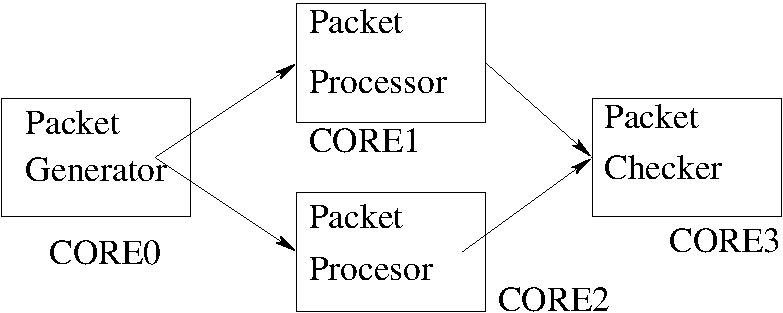
\includegraphics[width=10cm]{./figures/Niral_Router.pdf}
				\caption{Router software's structure}
				\label{app:router_soft}
			\end{figure}
		
		The figure~\ref{app:router_soft} shows brief structure of software. The system uses AJIT processor's timer to get the timings for packet processing.
		
		The average latency measured using 4x1x64 AJIT processor for 750 packets of size 90 bytes is \textbf{121.96} $\mu$s.











\end{appendices}

\iffalse
\begin{algorithm}
	\caption{Tmp alg template to use.}\label{alg:cap}
	\begin{algorithmic}
		\Require $n \geq 0$
		\Ensure $y = x^n$
		\State $y \gets 1$
		\State $X \gets x$
		\State $N \gets n$
		\While{$N \neq 0$}
		\If{$N$ is even}
		\State $X \gets X \times X$
		\State $N \gets \frac{N}{2}$  \Comment{This is a comment}
		\ElsIf{$N$ is odd}
		\State $y \gets y \times X$
		\State $N \gets N - 1$
		\EndIf
		\EndWhile
	\end{algorithmic}
\end{algorithm}
\fi